\documentclass[12pt,a4paper]{article}
\usepackage{natbib}
\usepackage{graphicx}
\usepackage{subcaption}
\usepackage{amsmath}
\usepackage{amsfonts}
\usepackage{mathtools}
\usepackage{enumitem}
\usepackage{setspace}
\usepackage{adjustbox}
\usepackage{placeins}
\usepackage{booktabs}
\usepackage{makecell}
\usepackage{tabularx}
\usepackage{tabulary}
\usepackage{hyperref}
\usepackage[capitalise,noabbrev]{cleveref}
\usepackage[a4paper, total={6in, 9in}]{geometry}
\usepackage{tikz}
\usepackage{bm}
\usepackage{tocloft}
\usepackage[sc]{mathpazo}
\usetikzlibrary{shapes,arrows,positioning}

\renewcommand\cftlottitlefont{\large}
\renewcommand\cftloftitlefont{\large}

%\bibliographystyle{agsm}
\bibliographystyle{apalike}
\setcitestyle{authoryear,open={(},close={)}}

\newcommand{\pkg}[1]{{\fontseries{b}\selectfont #1}} 


\title{Composite trade share and energy intensity}
\author{S. Drake Siard\\
MSc Economics 2019-2020 Dissertation}
\date{}

\linespread{1.25}
\begin{document}


\maketitle

\begin{abstract}
Declining energy intensity is a stylised fact common to nearly all economies, but its interactions with other economic factors are still a topic of active debate.
This paper builds on previous work examining the direct and indirect impacts of growth, industrialisation, technological innovation, urbanisation, and trade openness on energy intensity, focusing specifically on trade openness. 
We provide evidence that composite trade share, an alternate specification of trade openness, has a positive effect on energy efficiency, with an effect robust to using multiple specifications and country panel selections. 

Programs used: Python (\pkg{statsmodels}, \pkg{scipy}); R (\pkg{plm}, \pkg{pdynmc})

Word count: \emph{!! TODO !!}
 
\end{abstract}

\pagebreak

\tableofcontents

\pagebreak

\listoffigures
\listoftables

\pagebreak

\section{Introduction}\label{sec:introduction}

Energy intensity, defined as the total energy consumption per unit of economic output, is a critical measure of overall economic efficiency and sustainability.
For developing countries' economic growth to continue through this century without overwhelming the world's limited resources, their energy intensity must fall as their economies grow and they transition through the stages of industrialisation.
For the developed countries to maintain their quality of life while reducing their environmental impact, their transition to a post-industrial economy must be accompanied by decreasing energy use.
A better understanding of the drivers of energy intensity would benefit developed and developing nations alike.

One frequently recurring economic variable investigated in the literature on energy intensity is trade openness, often measured as the ratio of imports and exports to total economic activity.
There are several theoretical reasons why increased trade openness should lead to decreased energy intensity.
First, in developing nations increased integration into the world economy may increase penetration of technological innovation into domestic industries, increasing factor productivity.
Second, it may allow efficiency gains through substitution away from energy-intensive domestic
inputs as well as a focus on higher-productivity exports. 
However, increased trade may also allow developing nations with weaker environmental regulation to export high-pollution goods (effectively, importing pollution from developed nations). 
Unsurprisingly, the existing literature does not agree on either the sign or the significance of the empirical relationship.

This paper briefly explores the literature on trade openness and energy intensity (\cref{sec:literature}) and describes the economic variables in question more precisely in \cref{sec:data}.
The relationship is then empirically estimated using several linear dynamic panel data models, which are described and justified in \cref{sec:methodology}.
The detailed results of the analysis are presented in \cref{sec:results}, and \cref{sec:conclusion} summarises and concludes the paper.

\section{Literature Survey}\label{sec:literature}

\cite{ederAnalysisEnergyIntensity2018} describe the two most significant features of energy intensity. First, they describe its persistent downward trend across nearly all countries.
Second, despite widely varying initial levels of energy intensity and different energy intensity reduction rates, they demonstrate convergence of the series of energy intensity between economies.
We can take some comfort regarding future energy use from both of these features; however, as the authors note, the developing regions ``are not expected to reach the level of the economically developed countries by 2040" \citep[p.1971]{ederAnalysisEnergyIntensity2018}.
In addition, while useful for forecasting, such univariate analyses offer no information to policymakers wishing to accelerate the trend of energy intensity reduction. 
Analyses using decomposition methods, such in \cite{liuEightMethodsDecomposing2003}, can attribute changes in aggregate energy intensity to changes in total production, sectoral energy intensity and sector production share. While these could guide industrial policy aimed at rebalancing between sectors to achieve the desired effect, they still leave the open the question of which underlying factors affect energy intensity.

\cite{panHowIndustrializationTrade2019} begin with a broad survey of the literature on energy intensity and extract four commonly described determinants of energy intensity: economic growth, industrialisation, trade openness, and technological innovation.
They also cite a number of models and analyses that attempt to estimate the effect of these variables, noting that many such analyses explore only direct impacts of these factors, whereas interdependence between macroeconomic variables means many may have only indirect impacts on energy intensity, and the interactions may be bidirectional.
Finally, they propose a path model (a subset of recursive structural equation models) to analyse both the direct and indirect effects, and apply it to the specific situation of Bangladesh, 1986-2015.
They find a negative direct impact of trade openness on energy intensity, as well as an indirect negative impact mediated via economic growth (trade openness positively affects growth, which in turn negatively affects energy intensity).
However, using a similar model, \cite{siardPathModelEnergy2020} fails to replicate their results, and finds no significant relationship between the two either in Bangladesh or in several other countries.
\cite{tibaIncomeTradeOpenness2018} use a similar structural equation modelling technique, with a larger selection of countries, but without investigating energy intensity; they are concerned instead with energy consumption per capita. 
They report an effect with mixed signs across countries: in their model trade openness causes increased energy consumption per capita in Sweden and Canada, and decreased energy consumption in Portugal and Spain.
Interestingly, they also find that the arrow of causality occasionally runs in the opposite direction: energy consumption per capita causes increased trade openness in Switzerland, and decrease trade openness in the United Kingdom.
Their results for panels of high- and middle-income countries both show that the relationship between trade openness to energy consumption is insignificant when considered in aggregate. 

\cite{shahbazDynamicLinksEnergy2013} introduce another variable, the provision of domestic credit to the private sector, as a proxy for financial development. Limiting their investigation to China and using an ARDL bounds testing approach, they find bidirectional causality and a significant positive relationship between trade openness and energy consumption per capita; however, also they do not investigate energy intensity.

\cite{kasmanCO2EmissionsEconomic2015} add urbanisation, measured as the share of the population living in urban areas, to their analysis.
They investigate the linkage between between energy consumption, carbon dioxide emissions, economic growth, trade openness and urbanization for a panel of new EU member and candidate countries, using panel cointegration methods and panel causality tests.
Again, while not specifically addressing energy intensity, they find short-run unidirectional
causality running from increases in per capita energy consumption to increased trade openness, and not the other direction.

\cite{rafiqUrbanizationOpennessEmissions2016} investigate two generalisations of the above models: the Stochastic Impacts by Regression on Population, Affluence and Technology (STIRPAT) framework and the Environmental Kuznets Curve (EKC).
A summary and literature survey of the STIRPAT framework can be found in \cite{mcgeeImpactsTechnologyReevaluation2015}, but the general assumption of the model class is that measures of diverse anthropogenic environmental impacts, such as carbon dioxide emissions and diminished biodiversity, can be represented as a (multiplicative) function of population, affluence, and technology, using various proxies and measures for affluence and technology.
\cite{dindaEnvironmentalKuznetsCurve2004} provide a summary and literature survey of the EKC framework. 
The EKC hypothesis adds a non-linearity to the analysis by postulating a positive relationship between environmental impact and affluence at low levels, changing to a negative relationship as countries reach a suficient stage of development; the curve in question is stylistically represented as an inverted U-shape.

In their investigation, \cite{rafiqUrbanizationOpennessEmissions2016} examine the effect of trade openness on emissions and energy intensity in urbanising emerging economies in both STIRPAT- and EKC-type models.
Noting that their panel consists of countries from substantially different economic, social,
and cultural backgrounds, they use three linear (and one nonlinear) heterogenous panel estimation techniques.
The three linear estimators of the heterogeneous slope coefficients are the ``mean group estimator" of \cite{pesaranRoleEconomicTheory1997} and \cite{pesaranEstimatingLongrunRelationships1995}, the ``Common Correlated Effects Mean Group" (CCEMG) estimator from \cite{pesaranEstimationInferenceLarge2006}, 
and the ``Augmented Mean Group" (AMG) of \cite{eberhardtCrosssectionDependenceNonstationary2009} and \mbox{\cite{eberhardtProductivityAnalysisGlobal2010}}.
The non-linear estimator is that of \cite{kapetaniosNonlinearPanelData2014}.
They find that trade openness significantly reduces energy intensity in all four of the heterogenous panel
analyses that they apply, and verify the robustness of their results against endogeneity among the regressors with the GMM panel estimation of \cite{arellanoTestsSpecificationPanel1991}.
\cite{koengkanPositiveImpactTrade2018} also use the \cite{arellanoTestsSpecificationPanel1991} estimator with a different model specification but some more comprehensive diagnostics; again, however, the sample set is quite limited (a set of 4 Andean countries) and the dependent variable is energy consumption, not energy intensity.

\cite{coleDoesTradeLiberalization2006}\footnotemark{} note that the effect of trade liberalization on energy intensity depends on whether countries are they are importers or exporters of energy intensive output, which in turn depends on comparative advantage, driven by factor endowments. 
They use a fixed-effect panel methodology to estimate a model with interactions, and find that trade is positively related to energy use.
However, the only economic variables in their model are the capital-labor ratio, energy intensity, and trade, where the capital-labor ratio stands as a proxy for overall relative factor abundance.
\footnotetext{Building on \citep{antweilerFreeTradeGood2001}, who lay out the economic justification for the model and apply the analysis to various air pollutants.}

Another contribution of \cite{coleDoesTradeLiberalization2006} to the literature is the introduction of an alternate measure of trade openness, based in their case on the gravity model of \cite{frankelEstimateEffectCommon2002}.
The naive measure of trade openness (the ratio of the sum of imports and exports to GDP) used in the previously cited papers is open to question, and \cite{fujiiWhatDoesTrade2019} provides a useful critique, finding that the between-country variation of the standard trade openness measure derives more from the variability in GDP than variability in trade.

\cite{squalliNewMeasureTrade2011} extend this critique, noting an interesting anomaly: that according to the naive measure, the world’s largest trading countries are ranked among the most closed to trade.
However, in many alternate measures taking GDP variation into account, small evidently open economies are then ranked as closed to trade.
They propose a new measure of trade openness as a two-dimensional concept.
The first dimension, measuring the proportion of a countries' total income that is linked to international trade, they label as trade share; this is what the traditional variable measures.
Their second dimension is intended to reflect countries' interaction and interconnectedness; they measure as the fraction of each country's contribution to global trade, which they label world trade share.
They combine these two to produce a measure they call composite trade share (CTS), which is the product of the trade share with a normalised world trade share (the exact formula is given later in \cref{sec:data}).

The relationship of the current paper to the existing literature given above can be summed up as follows: 
\begin{itemize}
\item We use as a base the final model (Model IV, EKC-type) given in \cite{rafiqUrbanizationOpennessEmissions2016}, with energy intensity as the dependent variable. We include trade openness, population density, urbanisation, and affluence as explanatory variables.
\item We then add as further explanatory variables:
\begin{itemize}
\item technological innovation, as measured by total resident and non-resident patent application count, following \cite{panHowIndustrializationTrade2019}. 
However, rather than an absolute number, we use a per-capita metric, as in \cite{maradanaDoesInnovationPromote2017}
\item financial openness, as measured by the Chinn-Ito index \citep{chinnWhatMattersFinancial2006}, following \cite{koengkanPositiveImpactTrade2018}
\end{itemize}
\item We substitute the composite trade share metric of \cite{squalliNewMeasureTrade2011} as a measure of trade openness, rather than use the naive trade share of GDP.
\end{itemize}



\section{Data}\label{sec:data}
Where appropriate, we follow the naming convention of \cite{rafiqUrbanizationOpennessEmissions2016}, otherwise, we use abbreviations from the sources cited in \cref{sec:literature}.
The following variables were primarily drawn from the World Bank World Development Indicators database \citep{theworldbankWorldDevelopmentIndicators2020}:
\begin{itemize}
\item $ENI$ (energy intensity): total energy used, measured in kilograms of oil calorific equivalent, divided by gross domestic product, measured in current international dollars using purchasing power parity rates based on the 2017 ICP round \citep{theworldbankPurchasingPowerParities2020}.
The WDI field used is \texttt{EG.GDP.PUSE.KO.PP}, inverted, as the source data is supplied in GDP per unit of energy.
\item $POP$ (population density): midyear population, counting all residents, divided by land surface area in square kilometers. The WDI field used is \texttt{EN.POP.DNST}.
\item $AFL$ (affluence/GDP per capita): gross domestic product, measured in 2017 constant international dollars, divided by midyear population, counting all residents. The WDI field used is \texttt{NY.GDP.PCAP.PP.KD}.
\item $URB$ (urbanisation): population living in urban areas, divided by total population estimate. The WDI field used is \texttt{SP.URB.TOTL.IN.ZS}.
\item $TI$ (technological innovation): total annual patent application count per country, both directly and through the international patent process, by both residents and non-residents. The WDI fields used are \texttt{IP.PAT.RESD} and \texttt{IP.PAT.NRES}, which are added together, divided by \texttt{SP.POP.TOTL}.

Patent data was also retrieved directly from the WIPO Statistics Database via the IP Statistics Data Center, \cite{wipoWIPOStatisticsDatabase2020}, and used to fill in gaps in the WDI data where necessary; the field used was ``Total patent applications (direct and PCT national phase entries)".

The final value was scaled to represent the number of patents per 100,000 inhabitants.\footnote{A common scale in other innovation literature, e.g. \cite{ocampo-corralesKnowledgeFlowsTechnologies2020}.}
 
\end{itemize}
Trade openness is one measure of the integration of a country into the world economy. 
For a measure of trade openness, we replace the simple trade share measure ($OPN$ in \citealt{rafiqUrbanizationOpennessEmissions2016}) with the Comprehensive Trade Share  ($CTS$) measure of \cite{squalliNewMeasureTrade2011}.
This is constructed as follows:
\begin{enumerate}
\item The standard trade share ($TS$) for each country is formed by dividing the sum of imports ($M$) and exports ($X$) of good and services by GDP; this gives a measure of the importance of trade to that country's economy.
The corresponding fields from the WDI database are \texttt{NE.IMP.GNFS.CD}, \texttt{NE.EXP.GNFS.CD}, and \texttt{NY.GDP.MKTP.CD}.
In this case, we are using measures in current (2019) US\$, as the ratio then matches the values in the WDI database titled ``Trade (\% of GDP)" (\texttt{NE.TRD.GNFS.ZS}).
\item The world trade share ($WTS$) for each country is formed by dividing the country's trade by the total world trade. 
This gives a measure of that country's importance to world trade.
\item The composite trade share ($CTS$) is calculated by scaling the country's trade share $TS$ by the country's world trade share relative to the average world trade share across all countries.
\end{enumerate}

Explicitly, this can be written:
\begin{equation*}
TS_i = \frac{X_i + M_i}{GDP_i}
\qquad
WTS_i = \frac{X_i + M_i}{\sum_{j=1}^{n} ( X_j + M_j )}
\end{equation*}
\begin{equation*}
\overline{WTS} = \frac{\sum_{j=1}^{n} WTS_j}{n}
\qquad
CTS_i = \left( \frac{WTS_i}{\overline{WTS}} \right) TS_i
\end{equation*}
And can be simplified to:
\begin{equation}
CTS_i = \frac{X_i + M_i}{\frac{1}{n} \sum_{j=1}^{n} ( X_j + M_j )} \frac{X_i + M_i}{GDP_i}
\end{equation}
\cite{squalliNewMeasureTrade2011} carry out several robustness tests on the $CTS$ measure, and find it satisfactory; intuitively, it also succeeds in ranking both large trading countries (e.g. USA, Germany) and small open economies (e.g. Hong Kong, Singapore) highly, which neither $TS$ nor $WTS$ accomplish on their own.
We therefore substitute $CTS$ for $TS$ (denoted $OPN$ in the original model).

As another measure of financial integration into the world economy, we use the Chinn-Ito capital openness index, from \cite{chinnWhatMattersFinancial2006}.
This index, described in greater detail in \cite{chinnNewMeasureFinancial2008}, is based on the binary variables coding for financial restrictions supplied in the IMF's Annual Report on Exchange Arrangements and Exchange Restrictions (AREAER).
The value of the index is the first standardised principal component of the variables coding for the presence of multiple exchange rates, restrictions on current and capital account transactions, and export proceeds confiscations.
The direction of the index is the reverse of the variables, taking higher values in more financially open countries, with a mean of zero by construction.
We use the most recent update of the index, based on the data in \cite{imfAnnualReportExchange2019}, and notate it as $KAOPEN$.

\renewcommand{\arraystretch}{1.5}
\begin{table}[htbp]
\centering
\begin{tabulary}{\textwidth}{l l L} 
\toprule 
Measure & Economic variable & Description and units \\ [1ex] 
\midrule 
$ENI$ & Energy intensity & Primary energy use in kg. of oil equivalent per (current PPP-adjusted) \$US of GDP \\
$POP$ & Population density & Population per square kilometer of land \\ 
$AFL$ & Affluence & GDP measured in (current PPP-adjusted) \$US, divided by mid-year population estimate \\
$URB$ & Urbanisation & Population in urban areas as a fraction of total population \\
$TI$ & Technological innovation & Total number of patent applications (both direct and PCT national phase entries) divided by mid-year population estimate, scaled by 100k \\ 
$CTS$ & Trade openness & Total trade as \% of GDP, scaled proportionally to share of world trade \\
$KAOPEN$ & Capital openness & Composite measure of relative financial openness, a weighted sum of financial restriction indicators from the IMF 2019 AREAER \\
\bottomrule 
\end{tabulary}
\caption{Variable names and descriptions}
\label{tab:data_source}
\end{table}

These data definitions are summarised in \cref{tab:data_source}.
All of the included data series are sampled at an annual frequency, with a multi-year reporting lag, and are revised series (not point-in-time).

For the country selection, we replicate the two panels from \cite{tibaIncomeTradeOpenness2018}: one of high-income (p.805) countries and one of middle-income (p.807) countries.
For nearly all high-income countries and most middle-income countries, all data points are available over the date range of 1990 to 2015; the limiting factor is often $ENI$, which starts no sooner than 1990 for any country and ends in 2014 or 2015.
Restricting date ranges to data availability results in different observation periods for each country, yielding unbalanced panels.
The countries and their respective observation date ranges are specified in \cref{tab:countries}.

Note that we have excluded Venezuela and Algeria from the panel; the former has has too few valid observations and the latter has a short period of missing data mid-series for the number of patents.
This gives a panel of $n=22$ and $19 \leq T_i \leq 26$ (where necessary for our analyses, we will truncate this to 1996-2015, so that $T < N$).

\renewcommand{\arraystretch}{1}
\begin{table}[htbp]
\centering
\begin{subtable}{0.45\textwidth}
\centering
\begin{tabular}{ll}
\toprule
   Country & Date range \\
\midrule
 Argentina &  1990-2014 \\
    Brazil &  1990-2014 \\
  Bulgaria &  1994-2014 \\
     Chile &  1990-2015 \\
     China &  1990-2014 \\
  Colombia &  1994-2014 \\
  Malaysia &  1990-2014 \\
    Mexico &  1990-2015 \\
  Thailand &  1990-2014 \\
    Turkey &  1990-2015 \\
\bottomrule
\end{tabular}
\caption{Middle-income}
\end{subtable}
\begin{subtable}{0.45\textwidth}
\centering
\begin{tabular}{ll}
\toprule
        Country & Date range \\
\midrule
      Australia &  1995-2015 \\
         Canada &  1990-2015 \\
         France &  1990-2015 \\
        Germany &  1990-2015 \\
          Japan &  1990-2015 \\
    Netherlands &  1990-2015 \\
       Portugal &  1990-2015 \\
          Spain &  1990-2015 \\
         Sweden &  1990-2015 \\
    Switzerland &  1996-2014 \\
 United Kingdom &  1990-2015 \\
  United States &  1990-2015 \\
\bottomrule
\end{tabular}
\caption{High-income}
\end{subtable}
\caption{Country panels}
\label{tab:countries}
\end{table}

\cref{fig:data_dists} in \cref{sec:graph_appendix} shows histograms and kernel density plots of the data for the combined set of countries in both panels, along with p-values of \cite{dagostinoTestsDepartureNormality1973} normality tests.
Examining the distribution of the data, we find that the standard log-transformation of all but the $KAOPEN$ variable bring the distributions generally closer to normality in broad appearance (though still far from normal, statistically speaking) and bring all variables into roughly the same order of magnitude in scale.
$KAOPEN$ has already been normalised by construction, so we leave it unchanged.

For robustness checks, we also prepare an unbalanced panel of all countries that have at least ten years of consecutive observations of the variables of interest; those countries and their data ranges can be found in \cref{tab:all_countries}.

Our first exploratory analysis is to plot the timeseries of $\ln ENI$ (\cref{fig:ENI_timeseries}) and confirm the stylised facts outlined above.
We can see that for the vast majority of the countries in the panel, $ENI$ is following a similar log-linear trend, confirming both the downward path and convergence (in absolute terms).

\begin{figure}[htbp]
\centering
\begin{subfigure}{\textwidth}
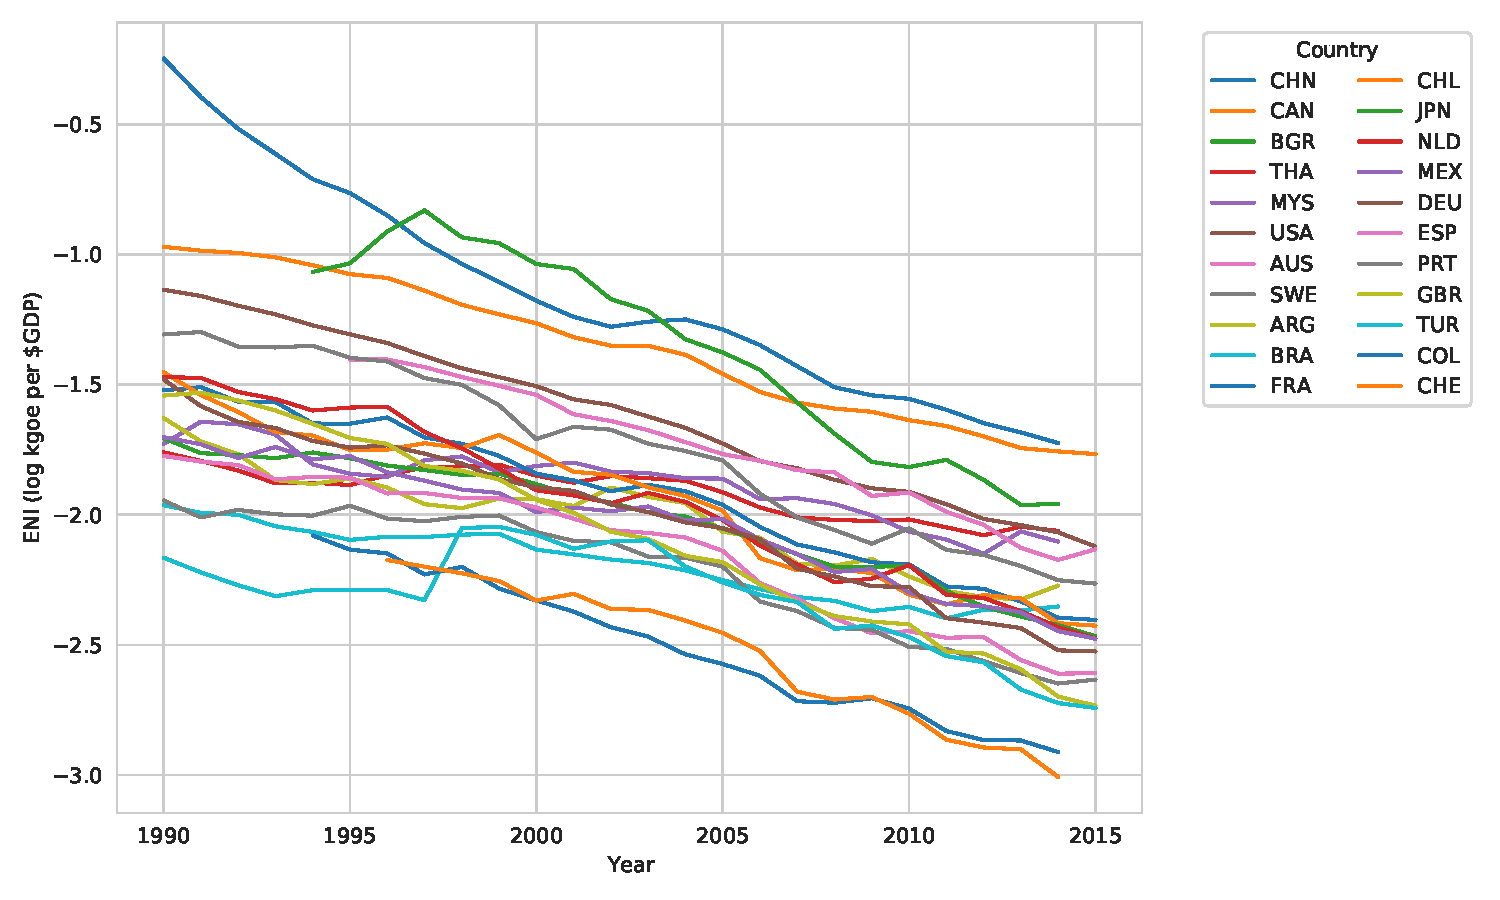
\includegraphics[height=10cm]{./plots/dis/timeseries_ENI_subset.pdf}
\caption{$\ln ENI$, restricted panel}
\end{subfigure}
\begin{subfigure}{\textwidth}
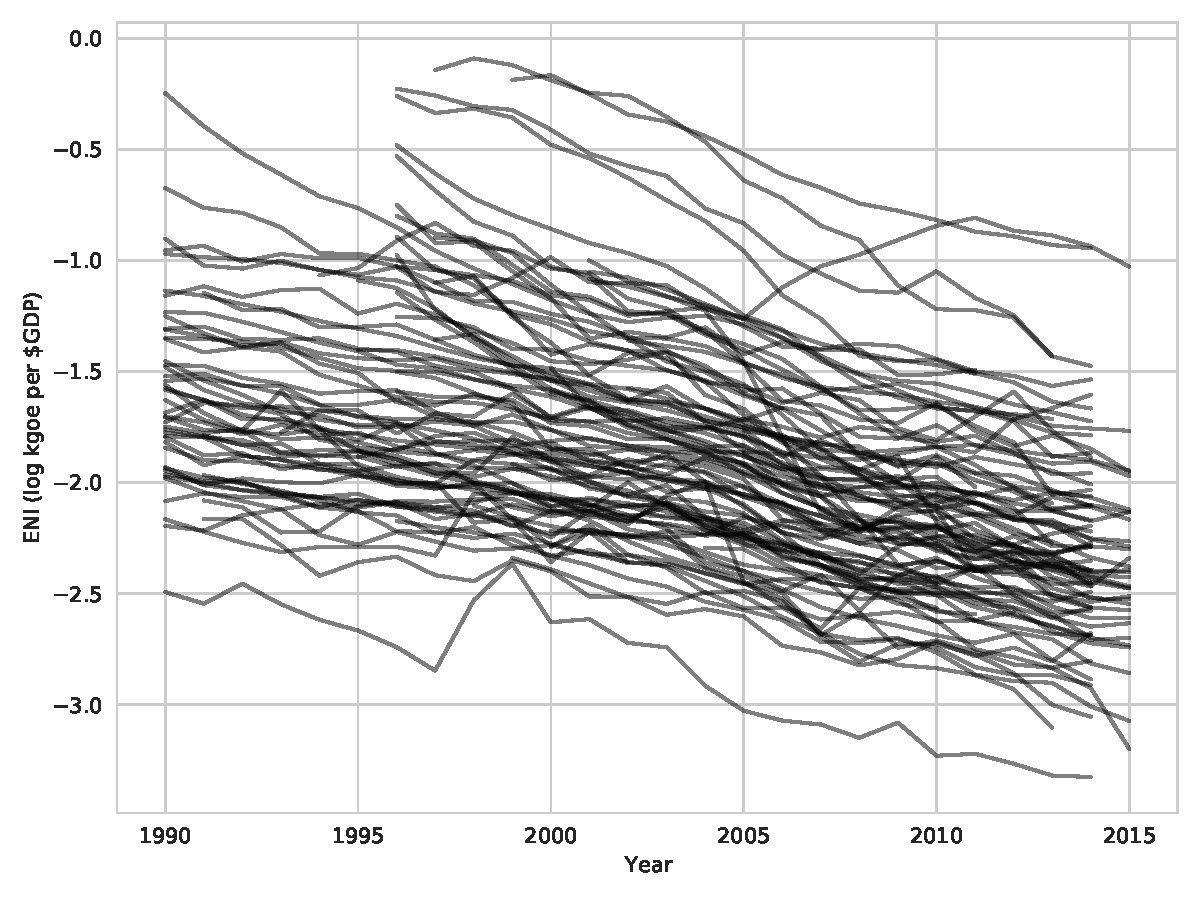
\includegraphics[height=10cm]{./plots/dis/timeseries_ENI_all.pdf}
\caption{$\ln ENI$, full panel}
\end{subfigure}
\caption{Energy intensity through time}
\label{fig:ENI_timeseries}
\end{figure}


Next, we check for non-stationarity in our data series. 
As we have an unbalanced panel, the Levin-Lin-Chu test of \cite{levinUnitRootTests2002} cannot be applied.
Instead, we use the cross-sectionally augmented\footnote{The standard version yields near-identical results, cross-section dependence is unlikely to be responsible for any difference.} version of the Im-Pesaran-Shin test of \cite{pesaranSimplePanelUnit2007}.
As time trends are apparent in the data, we apply the Case III ("trend") variant of the test.
The results of the test are found in \cref{tab:ips}; we fail to reject the null hypothesis of unit root for all tested variables.
However, applying the inverse chi-squared test of \cite{maddalaComparativeStudyUnit1999}, we get a completely different result, as can be seen in \cref{tab:madwu}.

\begin{table}[htbp]
\centering
\begin{subtable}{0.45\textwidth}
\centering
\begin{tabular}{llr}
\toprule
{} & statistic &      p-value \\
\midrule
ENI &     -1.68 &  $\geq 0.10$ \\
POP &     -1.30 &  $\geq 0.10$ \\
URB &     -1.60 &  $\geq 0.10$ \\
AFL &     -1.75 &  $\geq 0.10$ \\
TI  &     -1.86 &  $\geq 0.10$ \\
CTS &     -1.61 &  $\geq 0.10$ \\
\bottomrule
\end{tabular}


\caption{Im-Pesaran-Shin}
\label{tab:ips}
\end{subtable}
\begin{subtable}{0.45\textwidth}
\centering
\begin{tabular}{llr}
\toprule
{} & statistic &      p-value \\
\midrule
ENI &    103.22 &  $\leq 0.01$ \\
POP &    125.09 &  $\leq 0.01$ \\
URB &    343.22 &  $\leq 0.01$ \\
AFL &     77.88 &  $\leq 0.01$ \\
TI  &     70.23 &  $\leq 0.01$ \\
CTS &    156.45 &  $\leq 0.01$ \\
\bottomrule
\end{tabular}
\caption{inverse chi-squared}
\label{tab:madwu}
\end{subtable}
\caption{Panel unit root test results}
\end{table}

In summary, we have evidence both in support of and rejection of a unit root.
Fortunately, the dynamic panel models we propose in \cref{sec:methodology} allow for both the stationary and unit root case; the only assumption made regarding stationarity is that the process is not explosive \cite[p.5, A.2.1]{fritschGMMEstimationLinear2019}.

\clearpage
\section{Methodology}\label{sec:methodology}


The STIRPAT-inspired EKC-type model outlined at the end of \cref{sec:literature} combines the variables described in \cref{sec:data} in the following equation, where $i$ is country and $t$ is year:
\begin{multline}\label{eq:model}
\ln ENI_{it} = \delta_0 + \delta_1 \ln POP_{it} + \delta_2 \ln AFL_{it} + \delta_3 \left( \ln AFL_{it} \right)^2 + \delta_4 \ln URB_{it} \\ + \delta_5 \ln TI_{it} + \delta_6 \ln CTS_{it} + \delta_6 KAOPEN_{it} + \varepsilon_{it}
\end{multline}

Note that the specification for $AFL$ in \cref{eq:model} differs from \cite[Equation 4]{rafiqUrbanizationOpennessEmissions2016}, who have the following:
\begin{equation*}\label{eq:rafiqmodel}
\ln ENI_{it} = \delta_0 + \delta_1 \ln POP_{it} + \delta_2 \ln AFL_{it} + \delta_3 \ln AFL_{it}^2 + \delta_4 \ln URB_{it} + \cdots
\end{equation*}

This is, as others have diplomatically put it, "rather strange" \cite[p.4936]{moosaEconometricsEnvironmentalKuznets2017}, since $\ln AFL_{it}^2 = 2 \ln AFL_{it}$; however, as they go on to add, this would not be the first appearance of the $\ln \left( x^n_{it} \right)$ form in the literature.
In theory, the model of \cite{rafiqUrbanizationOpennessEmissions2016} cannot be estimated with ordinary procedures, as there is perfect colinearity between between the $\ln AFL_{it}$ and $\ln AFL_{it}^2$ terms, but looking into their data appendices\footnotemark{} we see that decimal truncation results in their corresponding \texttt{afl} and \texttt{afl2} fields being almost but not exactly collinear.

%TC:ignore
\urldef{\rafiqdata}\url{https://www.sciencedirect.com/science/article/pii/S0140988316300202?via%3Dihub#s0055}
%TC:endignore
\footnotetext{Available for download at \\
\begin{adjustbox}{max width=\textwidth}
\rafiqdata
\end{adjustbox}
}

Returning to \cref{eq:model}, there are many characteristics of the data that would prevent an ordinary least-squares estimation from returning consistent estimates.\footnote{
The following discussion draws from \cite{fritschGMMEstimationLinear2019} and \cite{rashidDynamicPanelData2018}.
}
First, omitted variable bias almost unavoidable when attempting to reduce the complexity of national economic systems to a handful of one-dimensional variables.
Potential endogeneity between our variable of interest and the regressors is a problem, as \cite{shahbazDynamicLinksEnergy2013} demonstrate in the case of trade and \cite{nayanRevisitingEnergyConsumption2013} cover in the case of growth; there is also likely to be endogeneity among the regressors, as \cite{rodriguezTradePolicyEconomic2001} demonstrate between trade and growth.
There is likely to be unobserved unit-specific heterogeneity, between countries from different economic, social, and cultural backgrounds.
In addition, there is also likely to be unobserved time-varying heterogeneity, as countries face common geopolitical, economic, and financial shocks, but with responses of varying degrees.
We can use the fact that we have multiple observations across both countries and time periods to model both dimensions of heterogeneity.
If we leave aside for a moment the time-heterogeneity, and assume common time-specific effects, the generalised construction of the linear dynamic panel data model can be described as:
\begin{align}
y_{i,t} &= \rho_1 y_{i,t-1} + \dots + \rho_p y_{i,t-p)} 
	+ \boldsymbol{x}^\prime_{i,t} \boldsymbol{\beta}_0 + \dots + \boldsymbol{x}^\prime_{i,t-q} \boldsymbol{\beta}_q 
	+ u_{i,t} \label{eq:panel} \\
u_{i,t} &= a_i + \lambda_t + \varepsilon_{i,t}
\end{align}
following the notation of \cite{fritschGMMEstimationLinear2019}, where $i$ and $t$ identify individuals and time periods, $y$ is the endogenous variable with up to $p$ lags, $\boldsymbol{x}$ are explanatory variables with up to $q$ lags, and the error term $u$ is composed of an individual-specific effect $a_i$, a time-specific effect $\lambda_t$ and an observation-specific  idiosyncratic remainder $\varepsilon_{i,t}$.

One of the most commonly applied estimators of dynamic panel data models of this form is known as the difference GMM estimator.
It is most often cited as \cite{arellanoTestsSpecificationPanel1991}, though, as has been often pointed out, it owes its origins to \cite{holtz-eakinEstimatingVectorAutoregressions1988}.
It acquired its name via its method of dealing with the individual-specific effect $a_i$ by differencing \cref{eq:panel}.
The underlying assumptions and corresponding moment conditions that extend the difference GMM into a family of models are laid out in detail in \cite{fritschGMMEstimationLinear2019}.
By assuming that first differences of instrument variables are uncorrelated with the fixed effects, futher moment conditions can be added, as in \cite{arellanoAnotherLookInstrumental1995} and \cite{blundellInitialConditionsMoment1998}.
This second estimator uses a system of two equations, one of the original levels and in addition to the differences, and is known as the system GMM.
In our case, we avoid system GMM due to the additional assumptions required, which can be intuitively understood as needing that the ``individuals sampled are not too far from steady states, in the sense that deviations from long-run means are not
systematically related to fixed effects" \cite[p.128]{roodmanHowXtabond2Introduction2009}.
The variety of countries at different levels of technological and economic development in our panel prevent us from being able to make assumptions of that kind.

While the additional instruments of extensions to the difference GMM can improve efficiency, this is a trade-off that may introduce bias.
\cite{bontempiImplementingStrategyReduce2015} review literature documenting a wide variety of problems with instrument proliferation in GMM estimation, primarily related to overfitting, especially where the instruments are weak.
In addition, specification tests for over-identifying restrictions, such as the commonly used Sargan-Hansen test of \cite{sarganEstimationEconomicRelationships1958} and \cite{hansenLargeSampleProperties1982}, are more likely to fail to reject the null of validity.
While recent innovations exist to address this issue, such as principal component analysis on the instrument matrix as in \cite{bontempiImplementingStrategyReduce2015}, the simple expedients of truncating the number of lags and ``collapsing" the blocks of the instrument matrix as in \cite{roodmanNoteThemeToo2009} remain two of the most effective and easily implemented.

The Stata package \pkg{xtabond2}, as described in \cite{roodmanHowXtabond2Introduction2009}, is possibly the most commonly used implementation of the difference GMM estimator.
For ease of integration with existing work we use the R packages \pkg{plm} as described in \cite{croissantPanelDataEconometrics2008} and \pkg{pdynmc} as described in \cite{fritschPdynmcPackageEstimating2019}.
We prefer to use \pkg{pdynmc} where possible as both slightly easier to use and better numerically behaved than \pkg{plm} when $T \rightarrow N$, as in our small panel case.
However, \pkg{plm} is the only one to support collapsing instruments and extracting certain fitted model variables for specification and goodness-of-fit-tests.

For GMM model verification, we use the Sargan-Hansen specification test described above for over-identifying restrictions. 
We also test model misspecification with the residual serial correlation test of \cite{arellanoTestsSpecificationPanel1991}.
When calculating standard errors of parameter estimates we rely on the finite sample variance correction of \cite{windmeijerFiniteSampleCorrection2005}, and for joint hypothesis testing against the null of zero parameters, we use the Wald test, whose statistic in this case is attributed to \cite{hayashiEconometrics2000}.

%TC:ignore

\vspace{1cm}
\noindent\textbf{TODO}
\begin{quote}
mtest.fct tests for serial correlation in the error terms \cite{arellanoTestsSpecificationPanel1991}


As a goodness of fit measure, we also present the squared correlation of , as in \cite{bloomUncertaintyInvestmentDynamics2007}.


"correction of Windmeijer 2005 was employed by this argument" https://cran.r-project.org/web/packages/pdynmc/vignettes/pdynmc.pdf
\end{quote}

\vspace{1cm}
\noindent\textbf{TODO}
\begin{quote}\cite{petrovicUnderlyingCausalFactors2018}
Dynamic panel data models: a guide to micro data methods and practice \cite{bondDynamicPanelData2002}


Democracy Does Cause Growth \cite{acemogluDemocracyDoesCause2019}


GMM Estimation from Incomplete and Rotating Panels \cite{albarranGMMEstimationIncomplete2019}
\end{quote}
%TC:endignore

\section{Results}\label{sec:results}


\cref{tab:diffgmm_coeff_subset}


\cref{tab:diffgmm_coeff_all} shows coefficient estimates and test results from the same models run on the extended panel over the same years.


\renewcommand{\arraystretch}{3}
\begin{table}[htbp]
\centering
\begin{tabular}{ccccccccc}
\toprule
                                               &                                 TS &                              TS+TI &                              TS+KO &                           TS+TI+KO &                                CTS &                             CTS+TI &                             CTS+KO &                          CTS+TI+KO \\
\midrule
                                         $POP$ &          \makecell{-0.857\\(0.36)} &          \makecell{-0.102\\(0.13)} &          \makecell{-0.760\\(0.18)} &   \makecell{-0.204***\\($< 0.01$)} &   \makecell{-0.278***\\($< 0.01$)} &   \makecell{-0.198***\\($< 0.01$)} &          \makecell{-0.037\\(0.32)} &          \makecell{-0.023\\(0.73)} \\
                                         $AFL$ &           \makecell{0.184\\(0.17)} &    \makecell{0.047***\\($< 0.01$)} &           \makecell{0.195\\(0.20)} &    \makecell{0.043***\\($< 0.01$)} &    \makecell{0.109***\\($< 0.01$)} &         \makecell{0.090**\\(0.03)} &           \makecell{0.033\\(0.53)} &           \makecell{0.042\\(0.68)} \\
                                       $AFL^2$ &        \makecell{-0.041**\\(0.02)} &   \makecell{-0.022***\\($< 0.01$)} &        \makecell{-0.040**\\(0.04)} &        \makecell{-0.015**\\(0.03)} &   \makecell{-0.034***\\($< 0.01$)} &   \makecell{-0.035***\\($< 0.01$)} &   \makecell{-0.034***\\($< 0.01$)} &   \makecell{-0.037***\\($< 0.01$)} \\
                                         $URB$ &          \makecell{-0.277\\(0.44)} &          \makecell{-0.001\\(0.99)} &          \makecell{-0.315\\(0.23)} &   \makecell{-0.040***\\($< 0.01$)} &   \makecell{-0.059***\\($< 0.01$)} &          \makecell{-0.003\\(0.86)} &           \makecell{0.058\\(0.73)} &           \makecell{0.026\\(0.82)} \\
                                          $TS$ &          \makecell{-0.049\\(0.80)} &           \makecell{0.168\\(0.28)} &           \makecell{0.024\\(0.93)} &         \makecell{0.415**\\(0.03)} &                                    &                                    &                                    &                                    \\
                                         $CTS$ &                                    &                                    &                                    &                                    &           \makecell{0.072\\(0.25)} &           \makecell{0.080\\(0.26)} &           \makecell{0.191\\(0.18)} &           \makecell{0.225\\(0.22)} \\
                                          $TI$ &                                    &           \makecell{0.028\\(0.12)} &                                    &           \makecell{0.017\\(0.21)} &                                    &         \makecell{0.033**\\(0.05)} &                                    &          \makecell{0.029*\\(0.07)} \\
                                      $KAOPEN$ &                                    &                                    &           \makecell{0.001\\(0.92)} &          \makecell{-0.005\\(0.51)} &                                    &                                    &           \makecell{0.003\\(0.87)} &           \makecell{0.001\\(0.98)} \\
              \makecell{Sargan-Hansen\\J-test} &        \makecell{0.13\\($> 0.99$)} &        \makecell{0.59\\($> 0.99$)} &        \makecell{0.03\\($> 0.99$)} &        \makecell{0.09\\($> 0.99$)} &        \makecell{0.37\\($> 0.99$)} &        \makecell{0.38\\($> 0.99$)} &        \makecell{0.02\\($> 0.99$)} &        \makecell{0.00\\($> 0.99$)} \\
                   \makecell{F-test\\(slopes)} &  \makecell{2656.44***\\($< 0.01$)} &  \makecell{3592.95***\\($< 0.01$)} &  \makecell{2747.66***\\($< 0.01$)} &  \makecell{4352.29***\\($< 0.01$)} &  \makecell{3663.40***\\($< 0.01$)} &  \makecell{3593.98***\\($< 0.01$)} &  \makecell{3408.58***\\($< 0.01$)} &  \makecell{3376.10***\\($< 0.01$)} \\
             \makecell{F-test\\(time dummies)} &   \makecell{275.58***\\($< 0.01$)} &   \makecell{452.83***\\($< 0.01$)} &   \makecell{326.76***\\($< 0.01$)} &   \makecell{834.53***\\($< 0.01$)} &   \makecell{299.15***\\($< 0.01$)} &   \makecell{368.52***\\($< 0.01$)} &   \makecell{358.83***\\($< 0.01$)} &   \makecell{426.96***\\($< 0.01$)} \\
 \makecell{Arellano-Bond\\ser. corr.  order 2} &          \makecell{2.41**\\(0.02)} &            \makecell{1.29\\(0.20)} &            \makecell{1.11\\(0.27)} &          \makecell{-1.83*\\(0.07)} &          \makecell{2.54**\\(0.01)} &          \makecell{2.06**\\(0.04)} &            \makecell{0.37\\(0.71)} &            \makecell{0.27\\(0.79)} \\
\bottomrule
\end{tabular}

\caption{Difference-GMM regression results, restricted panel}
\label{tab:diffgmm_coeff_subset}
\end{table}
\renewcommand{\arraystretch}{1}

\renewcommand{\arraystretch}{3}
\begin{table}[htbp]
\centering
\begin{tabular}{ccccc}
\toprule
                                               &                                   TS &                                  CTS &                               CTS+TI &                        CTS+TI+KAOPEN \\
\midrule
                                         $POP$ &            \makecell{-0.113\\(0.61)} &            \makecell{-0.145\\(0.53)} &            \makecell{-0.126\\(0.59)} &            \makecell{-0.114\\(0.64)} \\
                                         $AFL$ &             \makecell{0.353\\(0.43)} &             \makecell{0.225\\(0.64)} &             \makecell{0.214\\(0.65)} &             \makecell{0.173\\(0.73)} \\
                                       $AFL^2$ &          \makecell{-0.047**\\(0.05)} &           \makecell{-0.043*\\(0.08)} &           \makecell{-0.042*\\(0.08)} &            \makecell{-0.040\\(0.12)} \\
                                         $URB$ &             \makecell{0.072\\(0.83)} &             \makecell{0.115\\(0.76)} &             \makecell{0.125\\(0.75)} &             \makecell{0.145\\(0.71)} \\
                                          $TS$ &             \makecell{0.026\\(0.23)} &                                      &                                      &                                      \\
                                         $CTS$ &                                      &   \makecell{0.046***\\($\leq 0.01$)} &   \makecell{0.045***\\($\leq 0.01$)} &   \makecell{0.045***\\($\leq 0.01$)} \\
                                          $TI$ &                                      &                                      &            \makecell{-0.004\\(0.61)} &            \makecell{-0.004\\(0.64)} \\
                                      $KAOPEN$ &                                      &                                      &                                      &            \makecell{-0.004\\(0.51)} \\
              \makecell{Sargan-Hansen\\J-test} &             \makecell{77.47\\(1.00)} &             \makecell{77.73\\(1.00)} &             \makecell{77.64\\(1.00)} &             \makecell{77.17\\(1.00)} \\
                   \makecell{F-test\\(slopes)} &  \makecell{349.49***\\($\leq 0.01$)} &  \makecell{422.10***\\($\leq 0.01$)} &  \makecell{419.78***\\($\leq 0.01$)} &  \makecell{414.03***\\($\leq 0.01$)} \\
             \makecell{F-test\\(time dummies)} &   \makecell{58.93***\\($\leq 0.01$)} &   \makecell{60.63***\\($\leq 0.01$)} &   \makecell{60.99***\\($\leq 0.01$)} &   \makecell{61.14***\\($\leq 0.01$)} \\
 \makecell{Arellano-Bond\\ser. corr.  order 2} &              \makecell{1.17\\(0.24)} &              \makecell{1.09\\(0.28)} &              \makecell{0.89\\(0.37)} &              \makecell{0.87\\(0.39)} \\
\bottomrule
\end{tabular}

\caption{Difference-GMM regression results, all countries}
\label{tab:diffgmm_coeff_all}
\end{table}
\renewcommand{\arraystretch}{1}





\section{Conclusion}\label{sec:conclusion}

\clearpage

%TC:ignore
\appendix

\renewcommand{\refname}{\section{References}\label{sec:references}}.
\bibliography{project}

\clearpage

\newgeometry{margin=2cm}
\section{Appendices}

\subsection{Data and Code}\label{sec:data_and_code}

All of the data and code used to download and process it is available in the Github repository at the following URL:

\url{https://github.com/drakesiard/em-2020}

\noindent
The whole project may be downloaded at:

\url{https://github.com/drakesiard/em-2020/archive/v2.0.zip}

\noindent
The repository structure is described at:

\url{https://github.com/drakesiard/em-2020/blob/v2.0/README.md}

\noindent
All of the Python and R code and output are incorporated into Jupyter Notebooks, which have also been converted to HTML for ease of examination. For example, the FX analysis described in \cref{sec:data_analysis} can be found here:

\begin{adjustbox}{max width=\textwidth}
\url{https://htmlpreview.github.io/?https://github.com/drakesiard/em-2020/blob/v1.0/analysis/8_FX_impact.html}
\end{adjustbox}

\subsection{Additional Figures}\label{sec:graph_appendix}

\cref{fig:gmm_residual_plot}

\renewcommand{\arraystretch}{1}
\begin{table}[htbp]
\centering
\begin{subtable}{0.45\textwidth}
\centering
\begin{tabular}{ll}
\toprule
   Country & Date range \\
\midrule
                   Albania &  1995-2011 \\
                   Algeria &  1990-2007 \\
                 Argentina &  1990-2014 \\
                   Armenia &  2005-2014 \\
                 Australia &  1995-2015 \\
                   Austria &  1990-2015 \\
                Azerbaijan &  2001-2014 \\
                Bangladesh &  1990-2014 \\
                   Belarus &  1996-2014 \\
                   Belgium &  2000-2015 \\
                    Brazil &  1990-2014 \\
                  Bulgaria &  1994-2014 \\
                    Canada &  1990-2015 \\
                     Chile &  1990-2015 \\
                     China &  1990-2014 \\
                  Colombia &  1991-2014 \\
                   Croatia &  1996-2014 \\
                    Cyprus &  1999-2014 \\
                   Czechia &  1996-2015 \\
                   Denmark &  1990-2015 \\
        Dominican Republic &  2000-2014 \\
                   Ecuador &  1991-2010 \\
                     Egypt &  1998-2014 \\
                   Estonia &  1996-2015 \\
                   Finland &  1990-2015 \\
                    France &  1990-2015 \\
                   Georgia &  1996-2014 \\
                   Germany &  1990-2015 \\
                    Greece &  1990-2015 \\
                 Guatemala &  1990-2014 \\
                  Honduras &  2005-2014 \\
                 Hong Kong &  1990-2014 \\
                   Hungary &  1991-2015 \\
                   Iceland &  1990-2015 \\
                     India &  1990-2014 \\
                 Indonesia &  1991-2011 \\
					  Iran &  1993-2014 \\
                   Ireland &  1990-2015 \\
                    Israel &  1990-2015 \\
                     Italy &  1990-2015 \\
                   Jamaica &  2000-2014 \\
                     Japan &  1990-2015 \\
                    Jordan &  2000-2014 \\
                Kazakhstan &  1996-2011 \\
                     Kenya &  2002-2014 \\
\bottomrule
\end{tabular}
\end{subtable}
\begin{subtable}{0.45\textwidth}
\centering
\begin{tabular}{ll}
\toprule
        Country & Date range \\
\midrule
        Korea, Republic of &  1990-2015 \\
                Kyrgyzstan &  1997-2014 \\
                    Latvia &  1996-2014 \\
                 Lithuania &  1996-2014 \\
                  Malaysia &  1990-2014 \\
                     Malta &  1990-2002 \\
                    Mexico &  1990-2015 \\
                   Moldova &  1996-2014 \\
                   Morocco &  2004-2014 \\
                Mozambique &  1999-2014 \\
               Netherlands &  1990-2015 \\
               New Zealand &  1990-2015 \\
           North Macedonia &  1997-2013 \\
                    Norway &  1990-2015 \\
                  Pakistan &  1990-2014 \\
                    Panama &  2000-2014 \\
                  Paraguay &  2000-2010 \\
                      Peru &  1999-2014 \\
               Philippines &  1990-2014 \\
                    Poland &  1995-2015 \\
                  Portugal &  1990-2015 \\
                   Romania &  1990-2014 \\
        Russian Federation &  1996-2014 \\
              Saudi Arabia &  1990-2007 \\
                 Singapore &  1995-2014 \\
                  Slovakia &  1996-2015 \\
                  Slovenia &  1996-2011 \\
              South Africa &  1990-2014 \\
                     Spain &  1990-2015 \\
                 Sri Lanka &  1990-2013 \\
                    Sweden &  1990-2015 \\
               Switzerland &  1996-2015 \\
                Tajikistan &  1997-2006 \\
                  Tanzania &  2001-2011 \\
                  Thailand &  1990-2014 \\
                   Tunisia &  1990-2014 \\
                    Turkey &  1990-2015 \\
                   Ukraine &  1996-2014 \\
            United Kingdom &  1990-2015 \\
             United States &  1990-2015 \\
                   Uruguay &  1991-2012 \\
                Uzbekistan &  1997-2013 \\
                 Venezuela &  2002-2011 \\
                   Vietnam &  1990-2013 \\
                    Zambia &  2001-2013 \\
\bottomrule
\end{tabular}
\end{subtable}
\caption{Full width country panel}
\label{tab:all_countries}
\end{table}


\begin{figure}[htbp]
\centering
\begin{subfigure}{0.45\textwidth}
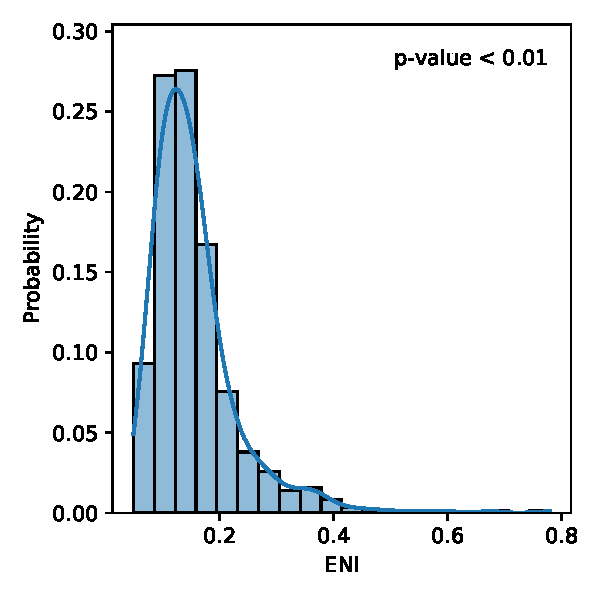
\includegraphics[width=\textwidth]{./plots/dis/distplot_ENI.pdf}
\caption{$ENI$}
\end{subfigure}
\begin{subfigure}{0.45\textwidth}
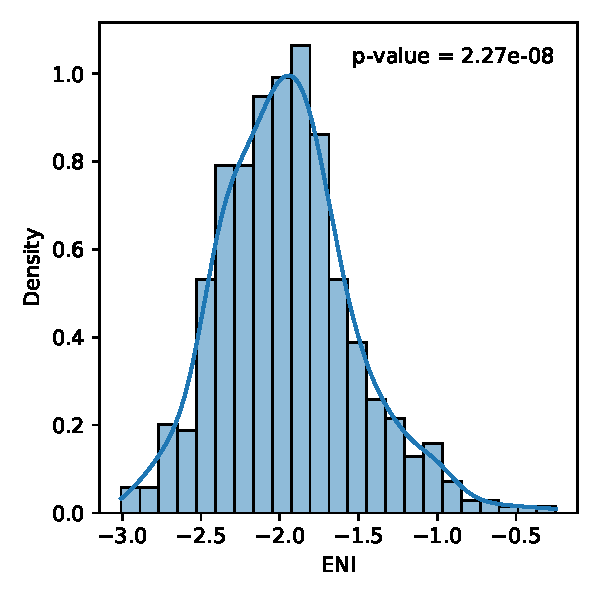
\includegraphics[width=\textwidth]{./plots/dis/distplot_lnENI.pdf}
\caption{$\ln ENI$}
\end{subfigure}
\begin{subfigure}{0.45\textwidth}
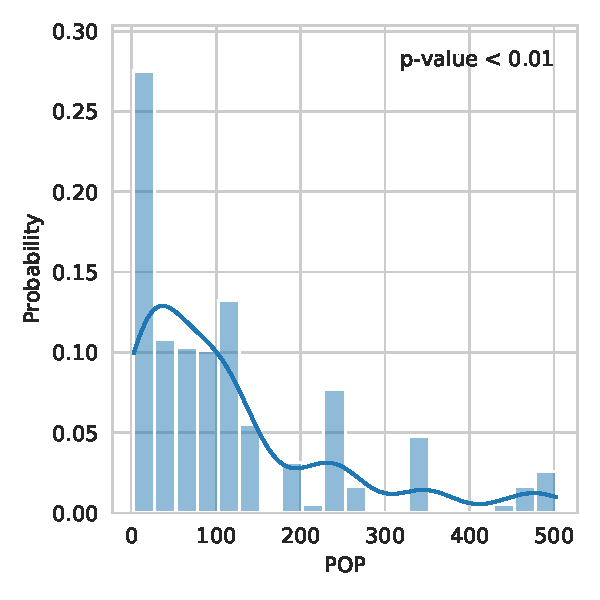
\includegraphics[width=\textwidth]{./plots/dis/distplot_POP.pdf}
\caption{$POP$}
\end{subfigure}
\begin{subfigure}{0.45\textwidth}
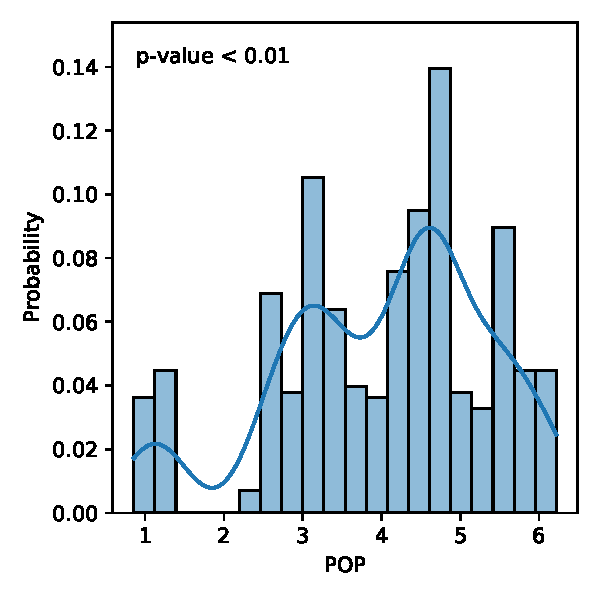
\includegraphics[width=\textwidth]{./plots/dis/distplot_lnPOP.pdf}
\caption{$\ln POP$}
\end{subfigure}
\begin{subfigure}{0.45\textwidth}
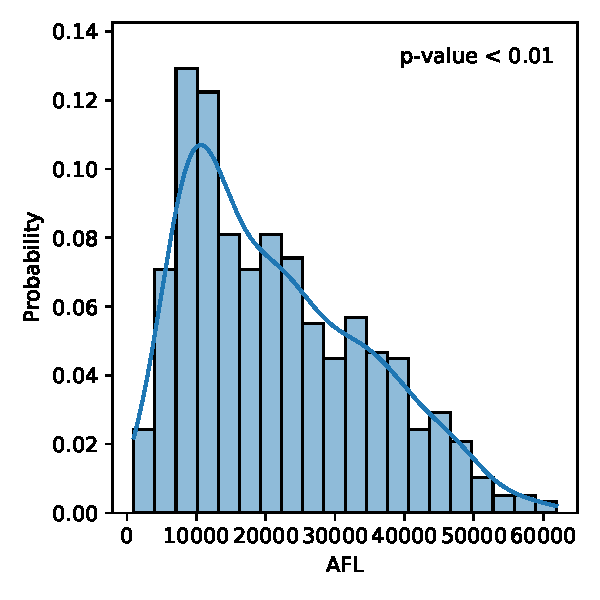
\includegraphics[width=\textwidth]{./plots/dis/distplot_AFL.pdf}
\caption{$AFL$}
\end{subfigure}
\begin{subfigure}{0.45\textwidth}
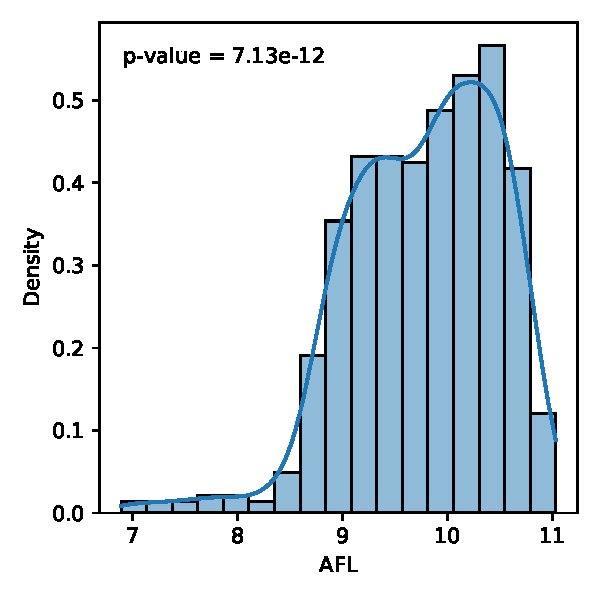
\includegraphics[width=\textwidth]{./plots/dis/distplot_lnAFL.pdf}
\caption{$\ln AFL$}
\end{subfigure}
\caption{Data histograms and density plots}
\label{fig:data_dists}
\end{figure}

\begin{figure}[htbp]\ContinuedFloat
\centering
\begin{subfigure}{0.45\textwidth}
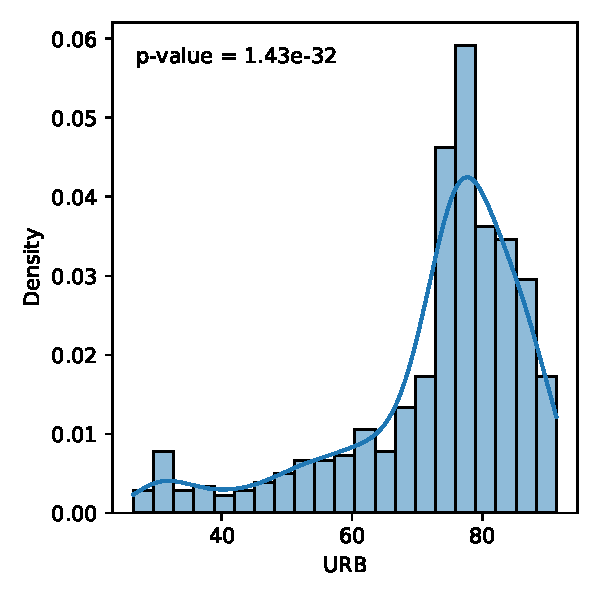
\includegraphics[width=\textwidth]{./plots/dis/distplot_URB.pdf}
\caption{$ENI$}
\end{subfigure}
\begin{subfigure}{0.45\textwidth}
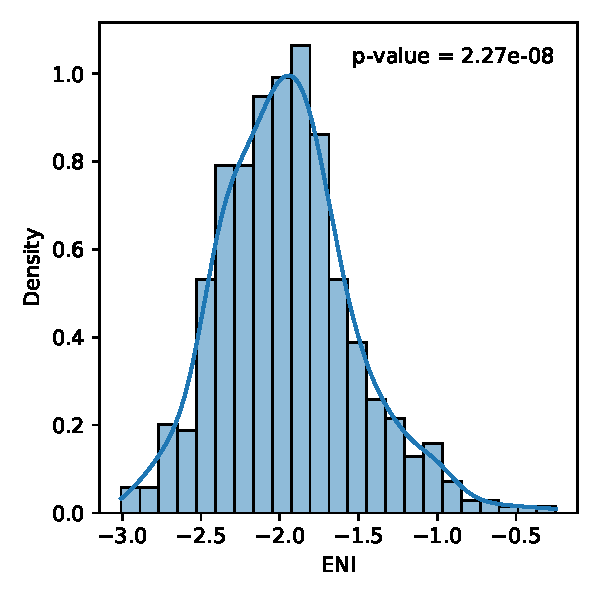
\includegraphics[width=\textwidth]{./plots/dis/distplot_lnENI.pdf}
\caption{$\ln ENI$}
\end{subfigure}
\begin{subfigure}{0.45\textwidth}
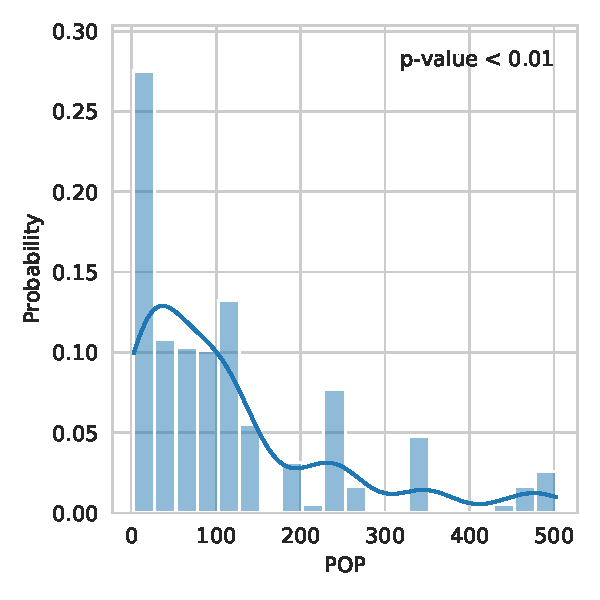
\includegraphics[width=\textwidth]{./plots/dis/distplot_POP.pdf}
\caption{$POP$}
\end{subfigure}
\begin{subfigure}{0.45\textwidth}
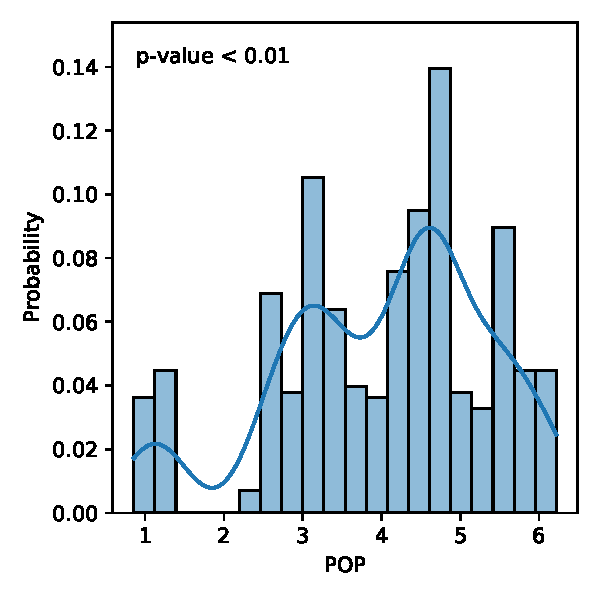
\includegraphics[width=\textwidth]{./plots/dis/distplot_lnPOP.pdf}
\caption{$\ln POP$}
\end{subfigure}
\begin{subfigure}{0.45\textwidth}
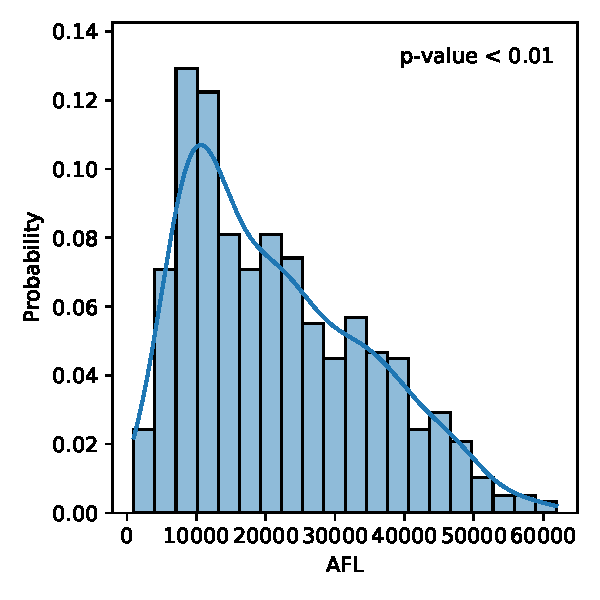
\includegraphics[width=\textwidth]{./plots/dis/distplot_AFL.pdf}
\caption{$AFL$}
\end{subfigure}
\begin{subfigure}{0.45\textwidth}
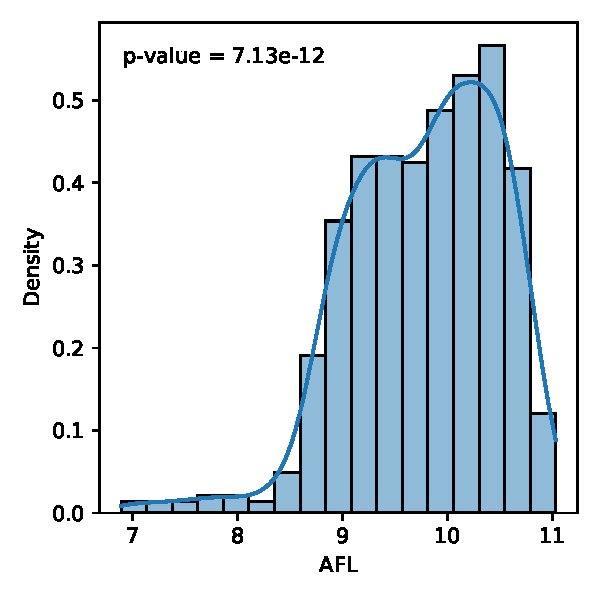
\includegraphics[width=\textwidth]{./plots/dis/distplot_lnAFL.pdf}
\caption{$\ln AFL$}
\end{subfigure}
\caption[]{Data histograms and density plots}
\end{figure}

\begin{figure}[htbp]\ContinuedFloat
\centering
\begin{subfigure}{0.45\textwidth}
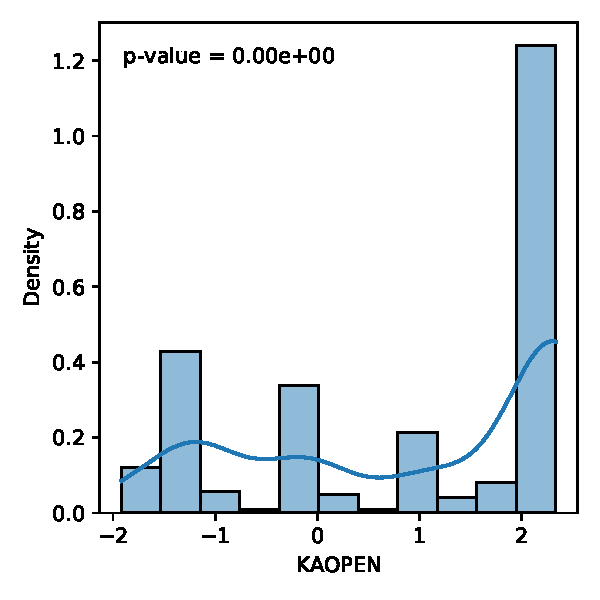
\includegraphics[width=\textwidth]{./plots/dis/distplot_KAOPEN.pdf}
\caption{KAOPEN}
\end{subfigure}
\caption[]{Data histograms and density plots}
\end{figure}

\FloatBarrier


\begin{figure}[htbp]
\centering
\begin{subfigure}{0.90\textwidth}
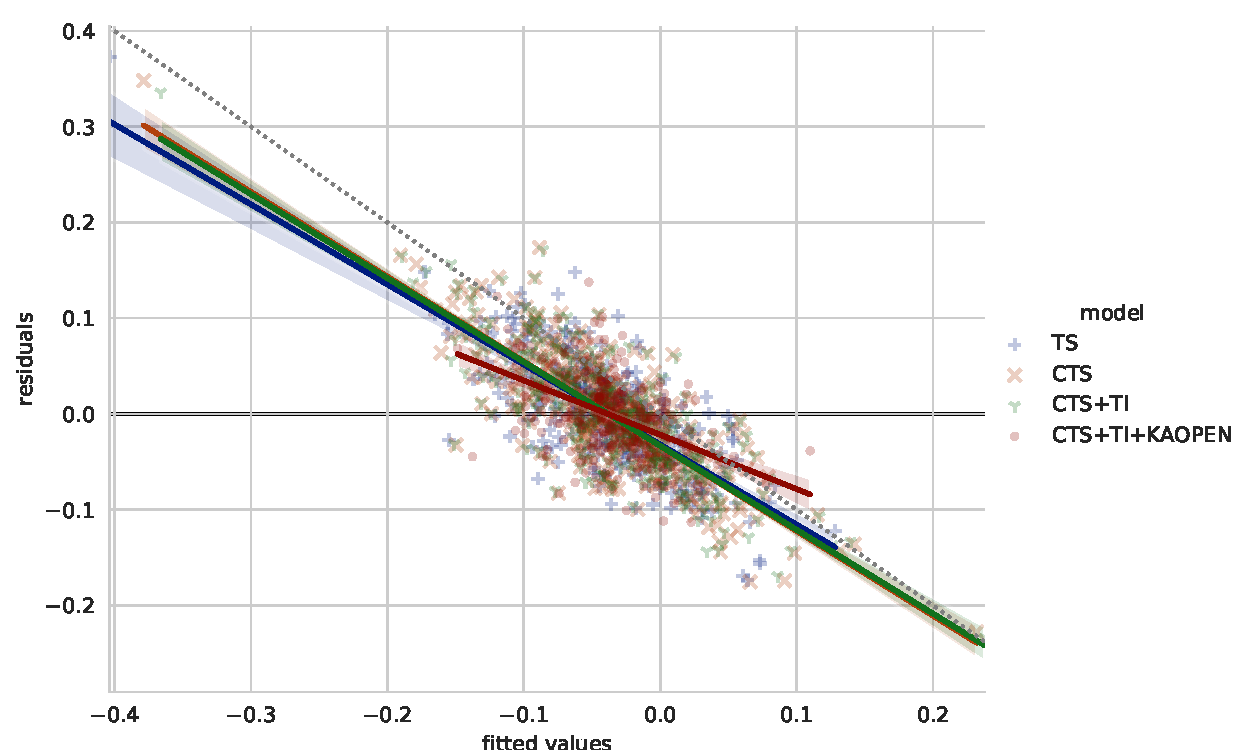
\includegraphics[width=\textwidth]{./plots/dis/diffGMM_residual_plot_subset.pdf}
\caption{Residual plot, restricted panel}
\end{subfigure}
\begin{subfigure}{0.90\textwidth}
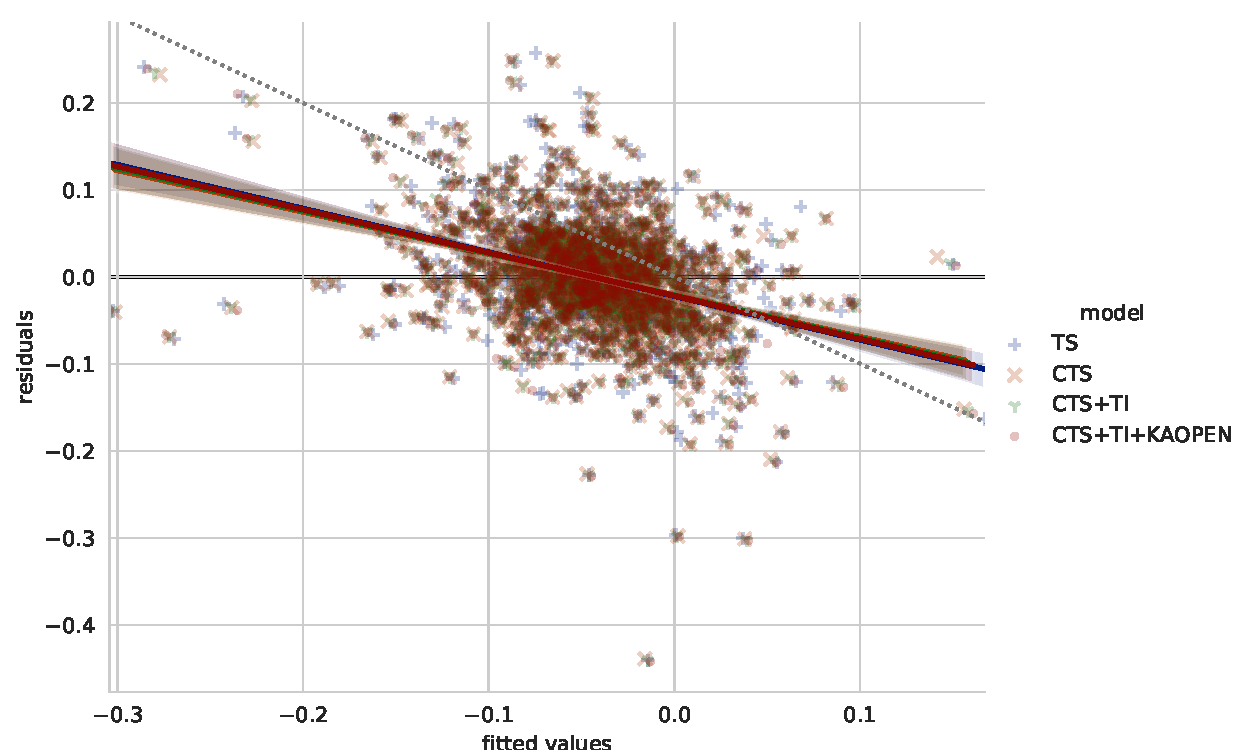
\includegraphics[width=\textwidth]{./plots/dis/diffGMM_residual_plot_all.pdf}
\caption{Residual plot, all countries}
\end{subfigure}
\caption{Residuals versus fitted values}
\label{fig:gmm_residual_plot}
\end{figure}



%TC:endignore
\restoregeometry{}

\end{document}